% beamer packages
\documentclass{beamer}[12pt]
\usetheme{boxes}
\usecolortheme{seahorse}
\beamertemplatenavigationsymbolsempty
\setbeamertemplate{footline}[frame number]
\setbeamertemplate{enumerate items}{arguments}

\usepackage{enumitem}

% graphics
\usepackage{tikz}
\usepackage{tkz-graph}
\usepackage{pgfplots}
\usepackage{xcolor}

% pseudocode
\usepackage{algorithmicx}
\usepackage[noend]{algpseudocode}

% maths
\usepackage{amsmath}
\usepackage{amsthm}

\newenvironment{claim}[1]{\par\noindent\underline{Claim:}\newline#1}{}
\renewenvironment{proof}[1]{\par\noindent\underline{Proof:}\newline#1}{}
\renewcommand{\qedsymbol}{}

\def\maxValue{1662}
\def\minValue{0}

\begin{document}
	\title{Presentation 2}
	\author{Fynn Lohren, Carsten Schubert, Leon Suchy}
	\date{\today}
	\frame{\titlepage}
	
	\begin{frame}
		\frametitle{Structure}
		\begin{itemize}[label={-}]
			\item Organisation
			\item Data Structures
			\item Lower Bounds
			\item Data Reduction
		\end{itemize}
	\end{frame}

	\begin{frame}
		\frametitle{Organisation}
		\begin{itemize}[label={-}]
			\item Issues on Gitlab to track open tasks
			\item Meeting with milestone goals
			\item Sick member\\
					$\rightarrow$ Less time than we wanted to have
		\end{itemize}
	\end{frame}
	
	\begin{frame}
		\frametitle{Data Structures}
		\begin{itemize}[label={-}]
			\item Heaps
			\item Bipartite Graph
			\item Controller
		\end{itemize}
	\end{frame}
	
	\begin{frame}
		\frametitle{Bipartite Graph}
		\begin{columns}[c]
			\column{.8\textwidth}
			\hspace{4mm}
			\begin{tabular}{|l|l|l|l|}\hline
				Index & Vertex ID & ID left & ID right \\ \hline \hline
				0 & 0 & 0 & \\ \hline
				1 & uint\_max - 1 & & 0 \\ \hline
				2 & 1 & 1 & \\ \hline
				3 & uint\_max - 2 & & 1 \\ \hline
				4 & 2 & 2 & \\ \hline
				5 & NULL & & - \\ \hline
			\end{tabular}
			\column{.6\textwidth}
			
			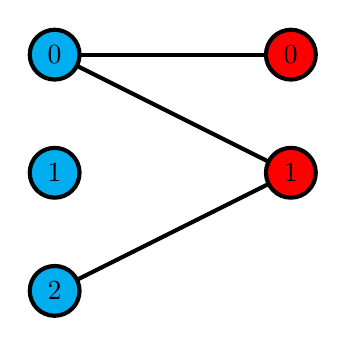
\begin{tikzpicture}
			%\draw[help lines] (0,0) grid (4,4);
			\SetVertexNormal[
			Shape 		= circle,
			LineWidth 	= 1.5pt]
			\SetUpEdge[
			lw 		= 1.5pt,
			color 	= black]
			
			\renewcommand{\VertexLightFillColor}{cyan}
			
			\Vertex[x=0,y=3,L=$0$]{0}
			\Vertex[x=0,y=1.5,L=$1$]{2}	
			\Vertex[x=0,y=0,L=$2$]{4}
			
			\renewcommand{\VertexLightFillColor}{red}
			\Vertex[x=3,y=3,L=$0$]{1}
			\Vertex[x=3,y=1.5,L=$1$]{3}
			
			\Edges(0,1)
			\Edges(0,3)
			\Edges(4,3)
			\end{tikzpicture}
		\end{columns}
	\end{frame}

	\begin{frame}
	\frametitle{Controller}
	\begin{itemize}[label={-}]
		\item Too much complexity synchronising all data structures
		\item Model/View/Controller pattern
	\end{itemize}
\end{frame}

	\begin{frame}
		\frametitle{Clique Cover LB Algorithm}
		\begin{algorithmic}[1]
			\Procedure{Clique Cover}{$G(V, E)$}
			\State $clique\_set \gets \{\}$
			\State $V \gets sort\_by\_degree(V)$ \Comment{Sort ascending}
			
			\ForAll {$v \in V$}
				\State $clique \gets largest\_clique(v)$ 
				\Comment{Largest clique v fits in}
				\State $clique\_set \gets clique\_set \setminus clique$
				\State $clique \gets clique \cup \{v\}$			
				\State $clique\_set \gets clique\_set \cup clique$	
			\EndFor
			\State 
			\Return $clique\_set$
			\EndProcedure
		\end{algorithmic}
		
		\vspace{3mm}
		Sorting can be computed in $\mathcal{O}(n \log{} n)$ time \\
		\pause
		Finding the largest clique for each v can be done in $\mathcal{O}(deg(v))$ time \\
		\pause
		More realistic in $\mathcal{O}(\log{} n)$ time\\
		\pause
		\text{Total running time: }\\
		$\mathcal{O}(n \log{} n)$
	\end{frame}
	
	\begin{frame}
		\frametitle{Clique Cover LB}
		\begin{figure}
			\begin{tikzpicture}
				\begin{axis}[
				width=0.8\textwidth,
				height=0.6\textwidth,
				grid,
				xlabel={$n$},
				ylabel={$k$},
				colorbar,
				colorbar style={
					ylabel=time in seconds,
					ylabel style={
						yshift=-7em
					}
				}]
				
				% \thisrowno needs to be used because it does not find the time key for some reason
				\addplot[only marks, color=black, mark=*, scatter] table[x={n}, y={k}, scatter src=\thisrowno{1}, col sep=comma]{clique_random.csv};
				\addplot[only marks, color=black, mark=*, scatter] table[x={n}, y={k}, scatter src=\thisrowno{1}, col sep=comma]{clique_dimacs.csv};
				\end{axis}
			\end{tikzpicture}
		\end{figure}
		
	\end{frame}
	
	\begin{frame}
		\frametitle{Linear Programming LB Algorithm}
		%TODO explain the procedure, mention that we recompute the whole matching -> slow
		Hopcroft-Karp: Finds maximum matching in a bipartite graph
		\pause
		Achieved complexity: $ \mathcal{O} (m * \sqrt{n})$
		\pause
		\newline
		König theorem: \\
		Constructs minimum vertex cover from maximum matching in bipartite graph\\
		Theoretical complexity: $\mathcal{O} (m * \sqrt{n})$
	\end{frame}
	\begin{frame}
		\frametitle{LP bound construction}
		
		\begin{columns}
			\column{0.3 \textwidth}
		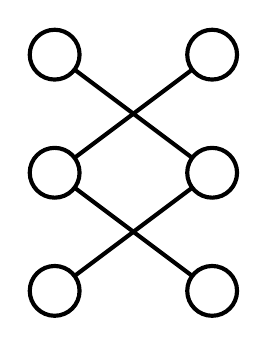
\begin{tikzpicture}
		%\draw[help lines] (0,0) grid (4,4);
		\SetVertexNormal[
		Shape 		= circle,
		LineWidth 	= 1.5pt]
		\SetUpEdge[
		lw 		= 1.5pt,
		color 	= black]

		
		\Vertex[x=0,y=3,L=$ $ ]{0}
		\Vertex[x=0,y=1.5,L=$ $]{2}	
		\Vertex[x=0,y=0,L=$ $]{4}
		

		\Vertex[x=2,y=3,L=$ $]{1}
		\Vertex[x=2,y=1.5,L=$ $]{3}
		\Vertex[x=2,y=0,L=$ $]{5}
		
		\Edges(2,1)
		\Edges(0,3)
		\Edges(4,3)
		\Edges(2,5)
		\end{tikzpicture}
		 \pause
		\column{0.3 \textwidth}
		 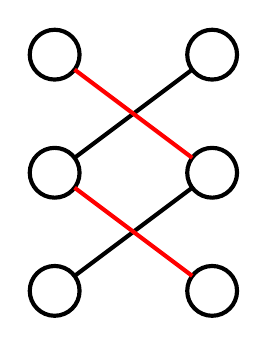
\begin{tikzpicture}
		 %\draw[help lines] (0,0) grid (4,4);
		 \SetVertexNormal[
		 Shape 		= circle,
		 LineWidth 	= 1.5pt]
		 \SetUpEdge[
		 lw 		= 1.5pt,
		 color 	= black]
		 
		 
		 \Vertex[x=0,y=3,L=$ $]{0}
		 \Vertex[x=0,y=1.5,L=$ $]{2}	
		 \Vertex[x=0,y=0,L=$ $]{4}
		 
		 
		 \Vertex[x=2,y=3,L=$ $]{1}
		 \Vertex[x=2,y=1.5,L=$ $]{3}
		 \Vertex[x=2,y=0,L=$ $]{5}
		 
		 \Edges(2,1)
		 \Edges[color=red](0,3)
		 \Edges(4,3)
		 \Edges[color=red](2,5)
		 \end{tikzpicture}
		 		 \pause
		 \column{0.3 \textwidth}
		 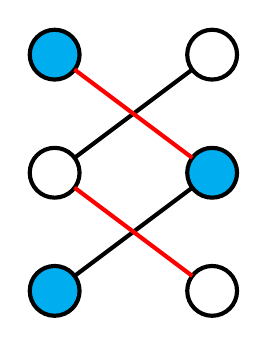
\begin{tikzpicture}
		 %\draw[help lines] (0,0) grid (4,4);
		 \SetVertexNormal[
		 Shape 		= circle,
		 LineWidth 	= 1.5pt]
		 \SetUpEdge[
		 lw 		= 1.5pt,
		 color 	= black]
		 
		 \Vertex[x=0,y=1.5,L=$ $]{2}	
		 \Vertex[x=2,y=3,L=$ $]{1}
		 \Vertex[x=2,y=0,L=$ $]{5}
		 
		\renewcommand{\VertexLightFillColor}{cyan}
		 
		 \Vertex[x=0,y=3,L=$ $]{0}

		 \Vertex[x=0,y=0,L=$ $]{4}
		 
		 

		 \Vertex[x=2,y=1.5,L=$ $]{3}

		 
		 \Edges(2,1)
		 \Edges[color=red](0,3)
		 \Edges(4,3)
		 \Edges[color=red](2,5)
		 \end{tikzpicture}
	\end{columns}
	\pause
	\vspace{8mm}
	$$VC = (L\setminus Z) \cup (R\cap Z)$$
	
	\end{frame}

	\begin{frame}
		\frametitle{Linear Programming LB}
		
		%TODO show the running time of linear programming lower bound in relation to k / n
		%TODO use the color encoding for time (see provided diagram example)
		\begin{tikzpicture}
			\begin{axis}[
				width=0.8\textwidth,
				height=0.6\textwidth,
				grid,
				ymax = 300,
				xlabel={$n$},
				ylabel={$k$},
				colorbar,
				colorbar style={
					ylabel=time in seconds,
					ylabel style={
						yshift=-7em
					}
				}]
				
				% \thisrowno needs to be used because it does not find the time key for some reason
				\addplot[only marks, color=black, mark=*, scatter] table[x={n}, y={Found VC}, scatter src=\thisrowno{1}, col sep=semicolon]{only_lp_bound_random_out.csv};
				\addplot[only marks, color=black, mark=*, scatter] table[x={n}, y={Found VC}, scatter src=\thisrowno{1}, col sep=semicolon]{only_lp_bound_dimacs_out.csv};
				

			\end{axis}
		\end{tikzpicture}
	\end{frame}
	
	\begin{frame}
		\frametitle{Lower Bound Comparison}
		
		% TODO compare recursive steps of both algorithms
		
		\begin{tikzpicture}[scale=1]
			\begin{loglogaxis}[
				width=0.9\textwidth,
				height=0.55\textwidth,
				xlabel={Clique Cover bound},
				ylabel={LP bound},
				legend cell align=left,
				legend pos=north west,
				legend entries= {random,dimacs},
				xmin=1,
				ymin=1,
				xmax=1662,
				ymax=1662]
				% the actual data points:
				%\addplot[color=black, only marks, mark=+, samples=200,domain=\minValue:\maxValue] {x + 10*x*(rand)};
				% using it with real data requires a csv-file:
				\addplot[only marks,color=blue,mark=+] table [y={Recursive Steps LP}, x={Recursive Steps CC},col sep=semicolon] {bound_comparison.csv};
				
				\addplot[only marks,color=orange,mark=*] table [y={Recursive Steps LP}, x={Recursive Steps CC},col sep=semicolon] {bound_comparison_dimacs.csv};
				
				\addplot+[mark=none,black,domain=1:1662] {x};
				% helper lines 
				%\addplot[color=black] {x};
				%\addplot[dashed,color=black!75,domain=\minValue:\maxValue,samples=4] {5*x};
				%\addplot[dashed,color=black!75,domain=\minValue:\maxValue,samples=4] {0.2*x};
				%\addplot[dotted,color=black,domain=\minValue:\maxValue,samples=4] {25*x};
				%\addplot[dotted,color=black,domain=\minValue:\maxValue,samples=4] {0.04*x};
			\end{loglogaxis}
		\end{tikzpicture}
	\end{frame}
	
	\begin{frame}
		\frametitle{Combining Lower Bounds}
		\begin{figure}
			\begin{tikzpicture}
				\begin{axis}[
					width=0.8\textwidth,
					height=0.6\textwidth,
					grid,
					xlabel={$n$},
					ylabel={$k$},
					colorbar,
					colorbar style={
						ylabel=time in seconds,
						ylabel style={
							yshift=-7em
						}
					}]
					
					\addplot[only marks, color=black, mark=*, scatter] table[x={n}, y={k}, scatter src=\thisrowno{1}, col sep=comma]{both_random.csv};
					/pause
					\addplot[only marks, color=black, mark=*, scatter] table[x={n}, y={k}, scatter src=\thisrowno{1}, col sep=comma]{both_dimacs.csv};
				\end{axis}
			\end{tikzpicture}
		\end{figure}
	\end{frame}
	
	\begin{frame}
		\frametitle{Data Reduction}
		
		\begin{block}{\underline{Degree 0 Rule}}
			If there is an isolated vertex, remove it
		\end{block}
		
		\vspace{4mm}
		
		\begin{block}{\underline{Degree 1 Rule}}
			If there is a degree-1 vertex, remove it and take its neighbour into the cover
		\end{block}
		
		\vspace{4mm}
		
		\begin{block}{\underline{High Degree Rule}}
			If there is a vertex with degree greater than k, take it into the cover
		\end{block}
	\end{frame}

	\begin{frame}
		\frametitle{Reduction Algorithm}
		\begin{algorithmic}[1]
			\Procedure {Exhaustive Reduction}{G, k}
			\State $applied \gets false$
			\Repeat
				\State $apply\_deg\_0(G, k)$
				\State $applied \gets apply\_deg\_1(G, k)$
				\State $applied \gets apply\_high\_deg(G, k)$
			\Until {not applied}
			\State \Return {$G', k'$}
			\EndProcedure
		\end{algorithmic}
		
		Runs in $\mathcal{O}(k \cdot n)$
	\end{frame}
	
	\begin{frame}
		\frametitle{Data Reduction}
		Properties of the reduced graph G'(V', E')?
		
		\begin{itemize}[label={--}]
			\item $\forall v \in V' . deg(v) \leq k'$ 
			\item $\forall v \in V' . deg(v) \geq 2$
		\end{itemize}
	\end{frame}
	
	\begin{frame}
		\frametitle{Data Reduction}
		Properties of the reduced graph G'(V', E')?
		
		\begin{itemize}[label={--}]
			\item $\forall v \in V' . deg(v) \leq k' \leftarrow \text{upper bound}$  
			\item $\forall v \in V' . deg(v) \geq 2$
		\end{itemize}
		
		\vspace{10mm}
		\centering
		\Large Limit size of our instance G' to k'!
	\end{frame}
	
	\begin{frame}
		\frametitle{Upper bound on graph size}
		
		\begin{claim}
			If $\Delta(G') \leq k'$ and $|E'| > k^2$ there is no VC of size k or smaller
		\end{claim}
		\pause
		\begin{proof}
			Let S be a vertex cover of G'. \\
			Every $v \in S \text{ can cover at most k' edges}.$
			Furthermore $|S| \leq k$. Then S can cover at most $k^2$ edges.
		\end{proof}
	\end{frame}
	
	\begin{frame}
	\frametitle{Upper bound on graph size}
		\begin{claim}
			If $|E'| \leq k'^2, \text{ then } |V'| \leq k'^2$
		\end{claim}
		\pause
		\begin{proof}
			By Degree-0 and Degree-1, G' has minimum degree at least 2. \\
			By Handshake-Lemma $\sum\nolimits_{v \in V'} deg(v) = 2|E'| \leq 2k'^2$\\
			This implies $|V'| \leq k'^2$
		\end{proof}
		\\
		\pause
		\vspace{5mm}
		$\rightarrow \text{reduced instance of G is bounded by k}$ \\
		\vspace{4mm}
		To be specific:
		$|V'| + |E'| \subseteq \mathcal{O}(k'^2)$\\
		$\Rightarrow$ Lower bounds become parameterised in $k$
	\end{frame}
	
	\begin{frame}
		%TODO some conclusions and an outlook to what we will be doing
		\frametitle{Outlook on Future Improvements}
		
		\begin{itemize}
			\item[-] Updating matching in bipartite graph instead of recomputing
			\item[-] Finish implementing existing reduction rules
			\item[-] Developing more sophisticated reduction rules 
			\item 	$\rightarrow$ to tighten the bound on the graph size
			\item[-] Better branching rules
			\item[-] Improve project modularity
		\end{itemize}
		


		
	\end{frame}
	\begin{frame}
		\frametitle{Thanks for your attention}
		\centering	\Huge Questions?
	\end{frame}

\end{document}